\documentclass[aspectratio=169]{beamer}
\usetheme{Madrid}
\usepackage{comment}
\usepackage{ragged2e}
\usepackage{amsmath}
\usepackage{xcolor}
\usepackage{multirow}
\usepackage{multicol}
\usepackage{caption}
\usepackage{tikz}
\usetikzlibrary{shapes.multipart}
\usetikzlibrary{calc}
\usetikzlibrary{shapes, arrows, positioning}
\usetikzlibrary{decorations.pathreplacing}
\usetikzlibrary{patterns}
\usepackage{booktabs}
\usepackage[title]{appendix}
\usepackage{booktabs}
\usepackage{appendixnumberbeamer}
\setbeamertemplate{caption}[numbered]
\usepackage{hyperref}
\hypersetup{
	colorlinks=false,
	linkcolor=blue,
	filecolor=blue,      
	urlcolor=blue,
}
\usepackage{graphicx}
\usepackage{mathtools}
\usepackage{amssymb}
\usepackage{amsthm}
\usepackage{thmtools}
\usepackage{natbib}
\newtagform{nonums}[\phantom]{}{}
\usetagform{nonums}

\newcommand\scalemath[2]{\scalebox{#1}{\mbox{\ensuremath{\displaystyle #2}}}}

\def\boxit#1{%
	\smash{\color{red}\fboxrule=1pt\relax\fboxsep=2pt\relax%
		\llap{\rlap{\fbox{\vphantom{0}\makebox[#1]{}}}~}}\ignorespaces
}
\renewcommand{\today}{\ifcase \month \or January\or February\or March\or %
	April\or May \or June\or July\or August\or September\or October\or November\or %
	December\fi, \number \year} 





\AtBeginSection[]
{
	\begin{frame}[noframenumbering,]{Table of Contents}
		\scriptsize
		
			\tableofcontents[hideallsubsections,hideothersubsections,currentsection]

		
	\end{frame}
}	
\title{Resource Reallocation with Carbon Emission Policies}
\author{Seyyed Morteza Aghajanzadeh}
\date{\today}
\subtitle{}
\institute[SSE]{Stockholm School of Economics}

\begin{document}
\maketitle
\section{Motivation}
\begin{frame}{Motivation}\large 
	\begin{itemize}
		\item Climate is changing, and it is going fast
		\item Environmental policies are designed to reduce the emissions and Save the planet
		\pause
		\item Therefore, Governments intervene in the market to reduce the emissions
		\item This intervention could lead to 
			\pause
			\begin{itemize}
				\item[$\blacksquare$] Fall in inputs 
				\item[$\blacksquare$] Introduce new inputs
				\item[$\blacksquare$] Reallocation of resources 
			\end{itemize}
	\end{itemize}
	% Add the idea of estimating the elasticity of substitution between green and brown capital
\end{frame}


\begin{frame}{Research Question}
	\begin{itemize}
		\item This reallocation could transfer resources from high to low productivity firms.
		\item Which could lead to a fall in the output of the economy
		\item So, the question is: \textbf{What is the cost of environmental policies due to reallocation?}
	\end{itemize}
\end{frame}

\begin{frame}{Literature and Contribution}
	\begin{itemize}
		\item ESG and Environmental Policy 
		\begin{itemize}
			\item \cite{martinsson2024effect} estimate the effect of carbon tax on the emission intensity of firms
		\end{itemize}
		\item Misallocation and Reallocation
		\begin{itemize}
			\item \cite{hsieh2009misallocation}
			\item \cite{whited2021misallocation}
		\end{itemize}
		\item Climate Policy Design
	\end{itemize}
	
\end{frame}

\section{Model}

\begin{frame}{Standard Framework}{\cite{hsieh2009misallocation}}
	\begin{itemize}
		\item Closed economy with heterogenous monopolistic competitive firms
		\item Production function is Cobb-Douglas 
		\item CES aggregator for the sector and economy-wide output
		\item Emission will be summed up to get the sector and economy-wide emission
	\end{itemize}
\end{frame}
\begin{frame}{Model}{Production function}
	\begin{equation}
		Y_{si} = \textcolor{blue}{\hat{A}_{si}}\textcolor{red}{\hat{K}_{si}}^{\beta_s} L_{si}^{1-\beta_s} \quad,\qquad \textcolor{red}{\hat{K} = (
			\alpha_s G_{si}^{\frac{\gamma_s-1}{\gamma_s}} + (1-\alpha_s) B_{si}^{\frac{\gamma_s-1}{\gamma_s}}
		) ^ {\frac{\gamma_s}{\gamma_s-1}}}
	\end{equation}

	\begin{equation}
		E_{si} = \textcolor{red}{\tilde{A}_{si}} B_{si}
	\end{equation}
	where 
	\begin{itemize}
		\item $\hat{A}_{si}$ is the total factor productivity
		\item $\tilde{A}_{si}$ is the emission intensity
		\item  $\alpha_s$ is the importance of Green capital in the production
		\item $\gamma_s$ is the elasticity of substitution between Green and Brown capital
	\end{itemize}
\end{frame}



\begin{frame}{Model}
	I have a closed monopolistic competition economy with firm heterogeneity:
	\begin{itemize}
		\item The real output for firms $i$ in sector $s$ is:
		 \begin{equation}
    \label{eq:firm_output}
    Y_{si} = \hat{A}_{si}\hat{K}_{si}^{\beta_s} L_{si}^{1-\beta_s}
    \quad,\qquad\hat{K} = (
        \alpha_s G_{si}^{\frac{\gamma_s-1}{\gamma_s}} + (1-\alpha_s) B_{si}^{\frac{\gamma_s-1}{\gamma_s}}
    ) ^ {\frac{\gamma_s}{\gamma_s-1}}
\end{equation}
			\pause
		\item The real output in each sector $s$ is:
			\begin{equation}
    Y_s = \left(
        \sum_{i=1}^I Y_{si}^{\frac{\sigma_s-1}{\sigma_s}}
    \right)^{\frac{\sigma_s}{\sigma_s-1}}
\end{equation}
		\item Total real output is:
			\begin{equation}
    Y = \Pi_1^S Y_s^{\lambda_s}, \quad \text{where} \quad \sum^S \lambda_s = 1
\end{equation}	
	\end{itemize}
\end{frame}

\begin{frame}{Model}
	\begin{itemize}
		\item The firm's emission is:
		\begin{equation}
    \label{eq:firm_emission}
    E_{si} = \tilde{A}_{si}\tilde{K}_{si}^{\theta_s} L_{si}^{1-\theta_s} \quad,\qquad \tilde{K} = (
        \mu_s G_{si}^{\frac{\eta_s-1}{\eta_s}} + (1-\mu_s) B_{si}^{\frac{\eta_s-1}{\eta_s}}
    ) ^ {\frac{\eta_s}{\eta_s-1}}
\end{equation}
		\pause
		\begin{itemize}
			\item It could be simplified as:
				\begin{equation*}
					E_{si} = \tilde{A}_{si}B_{si}
				\end{equation*}
			where $\mu_s = 0$ and $\theta_s = 1$.
		\end{itemize}
		\item The sector and economy-wide emission is defined as:
			\begin{equation}\label{eq:sector_emission}
    E_s = \sum_{i=1}^I E_{si}, \quad E = \sum_{s=1}^S E_s
\end{equation}
	\end{itemize}
\end{frame}

\begin{frame}{Model}
\begin{itemize}
	\item The nominal profit for firms:
	\begin{equation}
		\pi_{si} = {(1+\tau_{si}^p) P_{si} Y_{si} - \left(\left[
        (1+ \tau_{G_{s}}) r_{si}G_{si} + (1+ \tau_{B_{s}}) r_{si}B_{si} + (1+ \tau_{l_{s}}) w_{si}l_{si}
    \right] + {\tau_{E} E_{si}}\right)}
	\end{equation}
	\item To maximize the profit, first firm chooses the capitals and labor to minimize the cost of production and then chooses the price level.
	\item Then the firm chooses the optimal price level to maximize the profit.
\end{itemize}
\end{frame}

\begin{frame}{Model}{Optimal Allocation}
	\begin{equation*}
		\max  \quad
			- 		Cost \quad \text{s.t.} \quad \quad \hat{A}_{si}\hat{K}_{si}^{\beta_s} L_{si}^{1-\beta_s} = \bar{Y}_{si}
	\end{equation*}
	\begin{equation*}
	z^k_{si} \equiv \frac{G_{si}}{B_{si}} = \left[
    \frac{\alpha_s}{1-\alpha_s} \dfrac{\frac{\partial }{\partial B}Cost_{si}}{\frac{\partial }{\partial G}Cost_{si}}
\right] ^ {\gamma_s} 
	\end{equation*}
	\begin{equation*}
		\begin{split}
    z^l_{si} \equiv \frac{L_{si}}{\hat{K}_{si}} & = \frac{1-\beta_s}{\beta_s} \frac{1}{1-\alpha_s} (\alpha_s {z^k_{si}}^{(\gamma_s -1)} + (1-\alpha_s))^{\frac{1}{1-\gamma_s}}\dfrac{\frac{\partial }{\partial B}Cost_{si}}{\frac{\partial }{\partial L}Cost_{si}}\\
    & = \frac{1-\beta_s}{\beta_s} \frac{1}{\alpha_s}(\alpha_s  + (1-\alpha_s){z^k_{si}}^{(1-\gamma_s )})^{\frac{1}{1-\gamma_s}}\dfrac{\frac{\partial }{\partial G}Cost_{si}}{\frac{\partial }{\partial L}Cost_{si}}
\end{split}
	\end{equation*}
	
	\begin{equation}
    E_{si} = {\frac{\tilde{A}_{si}}{\hat{A}_{si}}(\frac{\phi_{si}}{z^{l}_{si}})^{\theta_s} {z^{l}_{si}}^{\beta_s}} \bar{Y}_{si} = \psi_{si}\bar{Y}_{si}, \quad \text{where} \quad \phi_{si}  = \frac{(\mu_s  + (1-\mu_s){z^k_{si}}^{(1-\eta_s )})^ {\frac{\eta_s}{\eta_s-1}}}{(\alpha_s  + (1-\alpha_s){z^k_{si}}^{(1-\gamma_s )}) ^{\frac{\gamma_s}{\gamma_s-1}}} 
\end{equation}
\end{frame}



% \begin{frame}{Model}{Cost function}
%     \begin{equation*}
    \begin{split}
        \Rightarrow C(\bar{F}_{si}) &  = \left[
            (1+ \tau_{G_{si}}) r^{G}_{si}G_{si} + (1+ \tau_{B_{si}}) r^{K}_{si}B_{si} + (1+ \tau_{l_{si}}) w_{si}l_{si}
        \right] + {\tau_{E} E_{si}} \\
        & = C_{si} \bar{F}_{si}  \\
    \end{split}
\end{equation*}
% \end{frame}
% \begin{frame}{Model}{Sector Price}
% 	\begin{itemize}
% 		\item We need to solve the sector price $P_s$ as function of firm price $P_{si}$, where $P_s$ is defined as the price of acquiring a unit of the sector benefit:
% 		\begin{equation*}
    \begin{split}
        \min_{F_{si}} & \quad \left\{
    \sum_{i} P_{si} F_{si}	
    \right\}\\
    \text{s.t.} & \quad \left(\sum_{i} F_{si}^{\frac{\sigma_s-1}{\sigma_s}}\right)^{\frac{\sigma_s}{\sigma_s-1}} = \bar{F}_s
    \end{split}
\end{equation*}
\begin{equation*}
    F.O.C \Rightarrow P_{si}^{\sigma_s} F_{si} = P_s^{\sigma_s} {F}_s
\end{equation*}
% 	\end{itemize}
	
% \end{frame}

\begin{frame}{Model}{Optimal firm level price}
	\begin{itemize}
		
		\item Now Firm need to choose the price level to maximize the profit:
		\begin{equation*}
    \max_{P_{si}} \quad \pi_{si} = P_{si}F_{si} - C_{si} {F}_{si}
\end{equation*}
		\item Firm-level real output is a function of the sector price, firm price, and sector real output (i.e. $F_{si} = (\frac{P_s}{ P_{si}})^{\sigma_s}{F}_s $)
		\item Therefore, because the optimal  ratio does not depend on the price, the ratio can be maximized out of the problem of the optimal determination of the price, leaving the firm’s real output as just a function of price
		\begin{equation}
    \begin{split}
         P_{si} =& \frac{1}{1+\tau_{si}^p}\frac{\sigma_s}{\sigma_s - 1} C_{si} \\
    \end{split}
\end{equation}
	\end{itemize}
\end{frame}

\section{Calibration}
\begin{frame}{Assumptions}
	\begin{itemize}
		\item First, I made some simplifying assumptions:
		\begin{itemize}
			\item $\mu_s = 0$
			\item $\theta_s = 1$
		\end{itemize}
		so the emission is:
		\begin{equation*}
			E_{si} = \tilde{A}_{si}B_{si}
		\end{equation*}
		\item Second, there is no friction in the market, so $\tau_{si}^p = \tau_{G_{si}} = \tau_{B_{si}} = \tau_{l_{si}} = 0$, now the profit is:
		\begin{equation*}
			\begin{split}
				\pi_{si} &=  P_{si} Y_{si} - (        r^{G}_{si}G_{si} + r^{B}_{si}B_{si} + w_{si}l_{si} + {\tau_{E} E_{si}})\\
				& = P_{si} Y_{si} - (r_{{si}}^GG_{si}  + (r_{{si}}^B + \tau_E\tilde{A}_{si})B_{si} +  w_{si}l_{si})
			\end{split}
		\end{equation*}
	\end{itemize}
\end{frame}
\begin{frame}{Calibration}{Table 2 in \cite{martinsson2024effect}}
	\begin{itemize}
		\item In order to use their table, I need to assume $\sigma = \infty$
		\item $\beta = 0.6$
		\item $r_B = r_G = 11\%$
		\item $1200$ firms in the same sector with different productivity levels which are drawn from a lognormal distribution.
		\item Firm level labor are drawn from a lognormal distribution with mean $250$ and standard deviation $900$.
		\item $W = 500,000$ SEK
	\end{itemize}
\end{frame}
\begin{frame}{Model equations}{Under assumptions}
	\input{model_elements/simplified model}
	Now I need to set the values of $\alpha_s$, $\gamma_s$, ${\hat{A}}$, and ${\tilde{A}}$ to match the summary statistics of Emission-to-sales ratio ($\sim 0.0072$), the elasticity of carbon tax on emissions' intensity ($\sim 2$) in \cite{martinsson2024effect}, and the total output in the economy ($\sim 10$ BSEK).
\end{frame}



\begin{frame}{Calibration results}
	\begin{figure}[http]
		\centering
		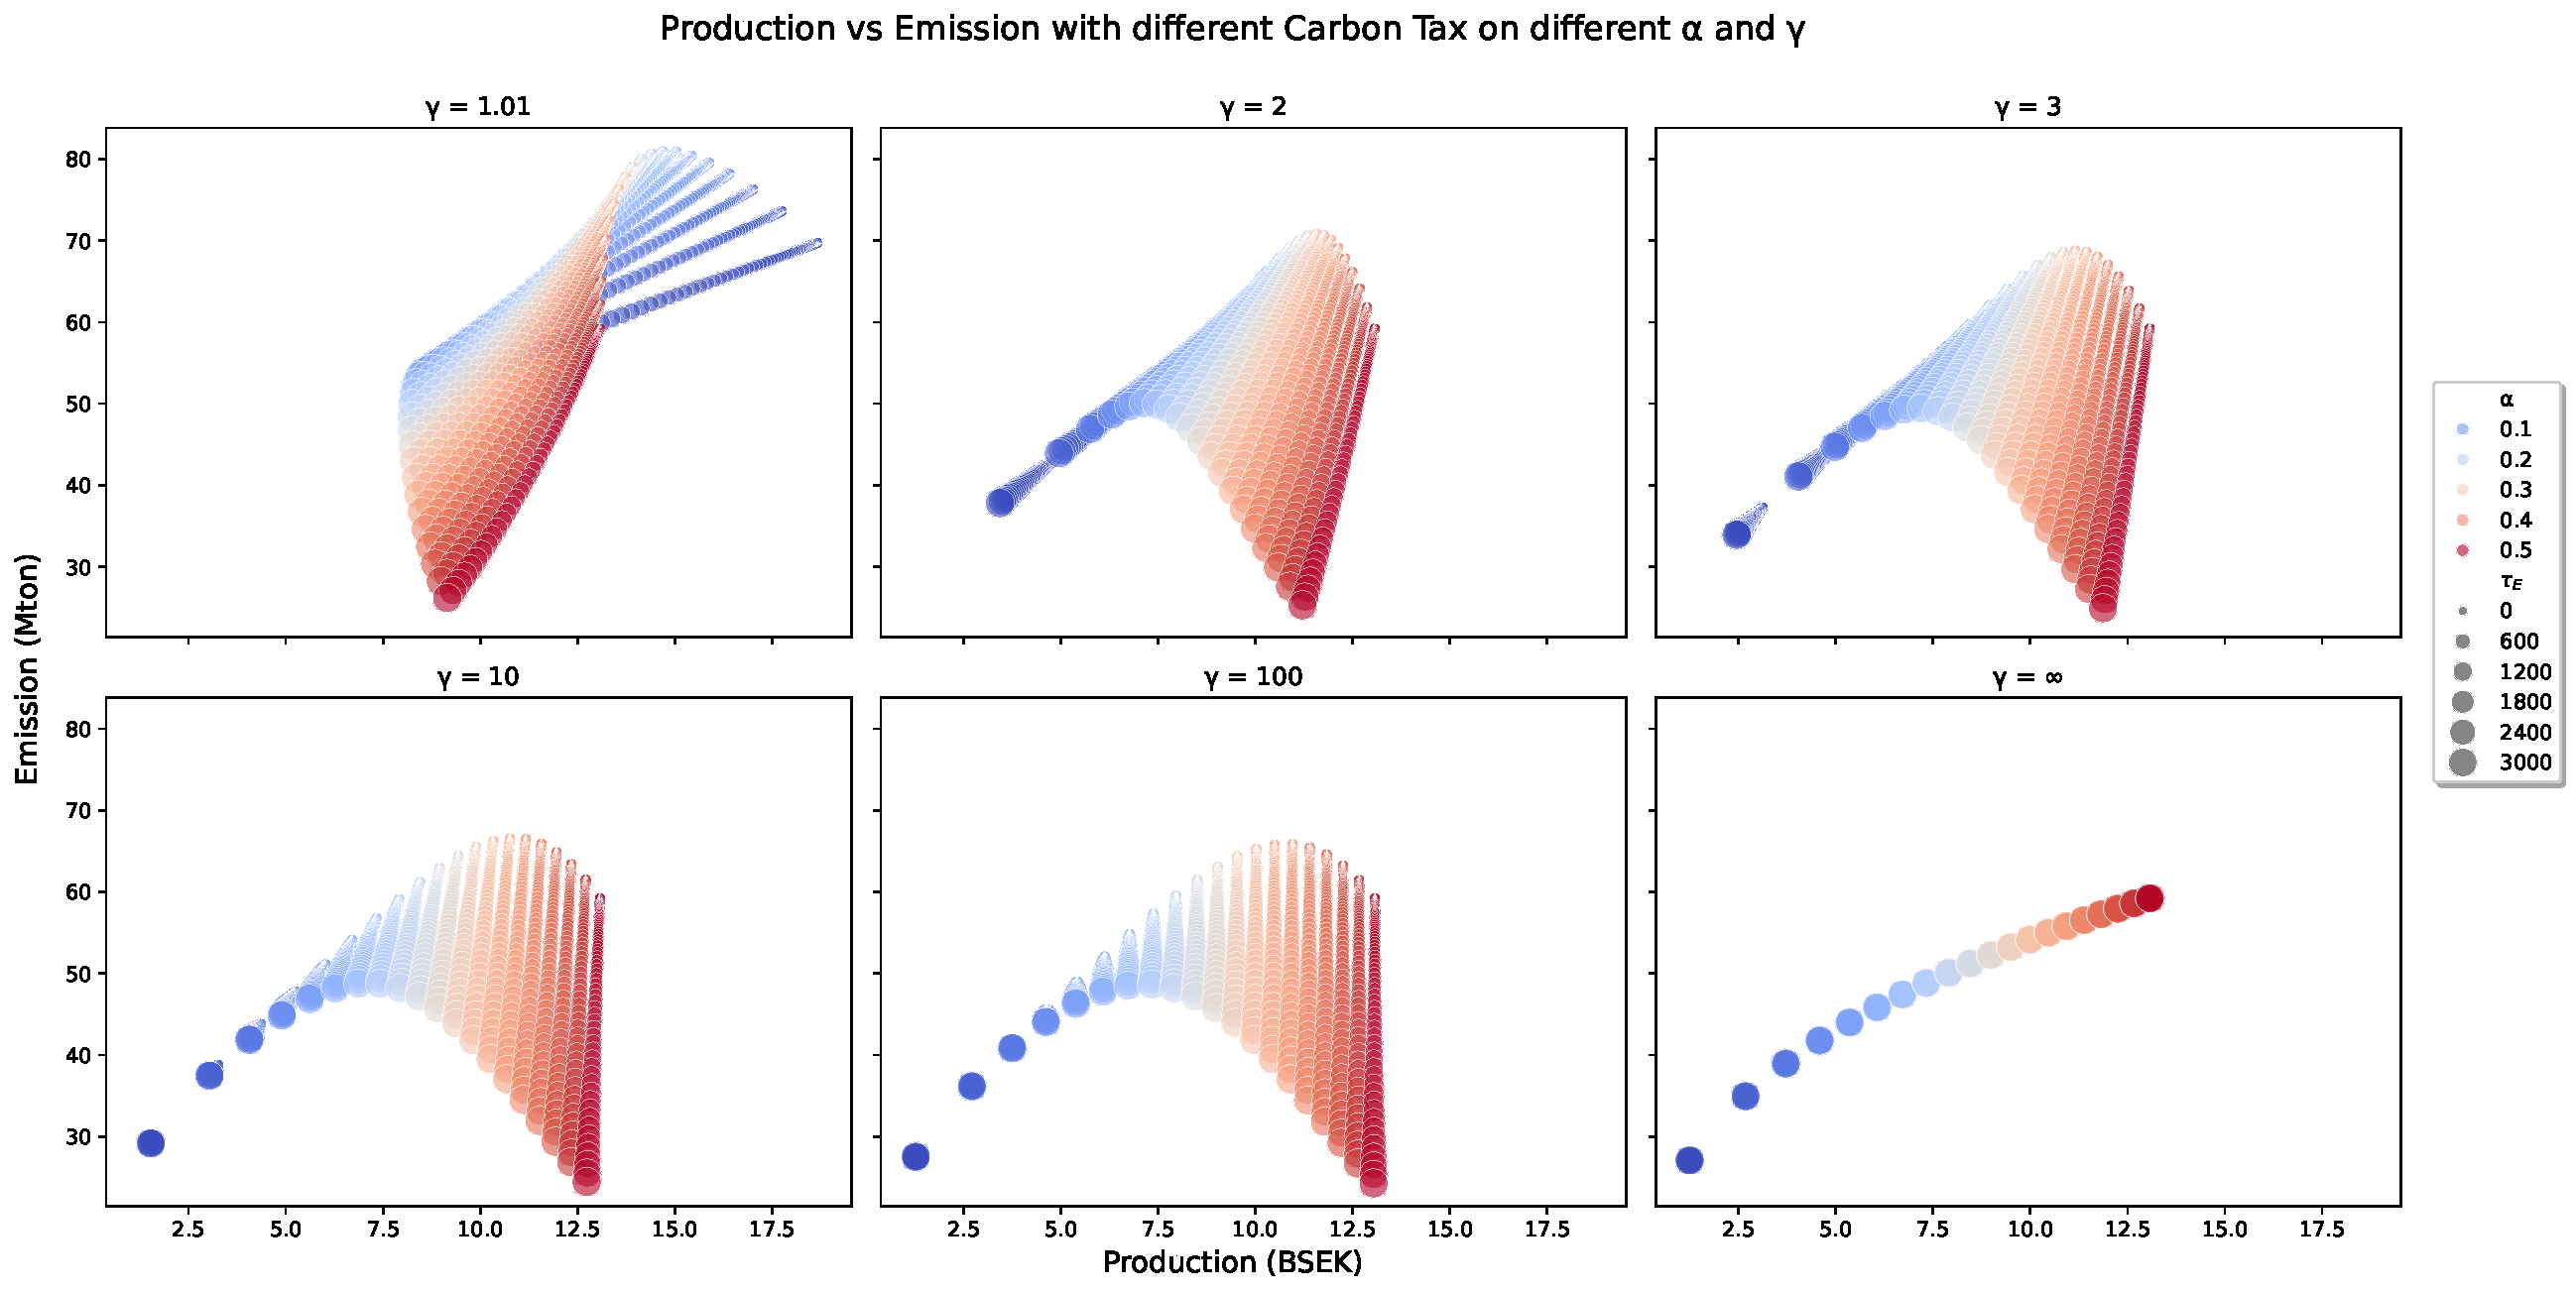
\includegraphics[width=0.9\textwidth]{Figures/production_emission.pdf}
	\end{figure}
\end{frame}

\begin{frame}{Calibration results}
	\begin{itemize}
		\item I need to have an average $\hat{A}=$ \input{values/A hat estimate} and $\tilde{A} =$ \input{values/A tilde estimate} to match the emission-to-sales ratio, and the total output ($\sim 10$ BSEK) in economy.
		\item I need to have $\alpha_s=$ \input{values/alpha estimate}, $\gamma_s = $ \input{values/gamma estimate} to match the elasticity of carbon tax on emissions' intensity.
	\end{itemize}
\end{frame}
\begin{frame}{Calibration results}
\begin{columns}
	\begin{columns}
		\begin{column}{0.7\textwidth}
			\begin{figure}[http]
				\centering
				\includegraphics<1->[width=\textwidth]{Figures/intensity_tax_premium.pdf}
			\end{figure}
		\end{column}
		\begin{column}{0.3\textwidth}
			\begin{table}
				{\begin{tabular}{ccc}
\toprule
$ \tau_E$ & $ \tau_G$ & $ \tau_B$ \\
\midrule
     100 &        9 \% &        2 \% \\
     250 &       18 \% &        2 \% \\
     500 &       27 \% &        4 \% \\
    1300 &       42 \% &       12 \% \\
    3000 &       55 \% &       26 \% \\
\bottomrule
\end{tabular}
}
			\end{table}
		\end{column}
	\end{columns}
\end{columns}
\end{frame}

\section{Reallocation}
% \begin{frame}{Reallocation}
% 	\begin{itemize}
% 		\item The real output is unobservable, making it difficult to calculate the gains from reallocation.
% 		\item To overcome this obstacle, the optimal allocations of Green and Brown capital are plugged into the firm-level CES aggregate to obtain the optimal firm-level.
% 		\item An estimate of the actual firm-level real output is calculated by plugging in the observed Green and Brown capital.
% 		\item The economy-wide real output is then calculated by aggregating the firm-level values into sectors and sectors into the aggregate economy, allowing for a comparison between the optimal and actual aggregated output to measure aggregate gains.
% 	\end{itemize}
% \end{frame}
\begin{frame}{Reallocation}
	\begin{itemize}
		\item Social planner's problem:
			\input{model_elements/social planner's problem}
		\item Lagrangian:
			\input{model_elements/social planner's problem - largranian}
	\end{itemize}
\end{frame}
% \begin{frame}{Reallocation}
% 	\begin{itemize}
% 		\item The optimal input ratios are:
% 			\begin{gather}\label{eq:reallocation_firm_input_ratio}
    z_{s}^k = (\frac{\alpha_s}{1-\alpha_s})^{\gamma_s} \\
    z_{s}^l = \frac{1-\beta_s}{\beta_s} \frac{1}{1-\alpha_s} (\alpha_s {z^k_{s}}^{(\gamma_s -1)} + (1-\alpha_s))^{\frac{1}{1-\gamma_s}} \lambda_L
  \end{gather}
% 		\item The optimal output and emissions for firm under the social planner's problem are:
% 			\input{model_elements/social planner's problem - firm output}
% 	\end{itemize}
% \end{frame}


\begin{frame}{Reallocation}{Resources allocation}
	\begin{itemize}
		\item Now, we need to find the optimal allocation of resources in the economy under two scenarios:
		\begin{columns}[T] % T aligns the columns from the top

			\begin{column}{0.5\textwidth} % First column
				\begin{gather} \label{eq:output_allocation_allocation}
    \hat{L}_{si} = \dfrac{\hat{A}_{si}^{\sigma -1}}{\sum_j \hat{A}_{sj}^{\sigma -1}}L_s\\ 
    \hat{G}_{si} = \dfrac{\hat{A}_{si}^{\sigma -1}}{\sum_j \hat{A}_{sj}^{\sigma -1}}\dfrac{z_s^k}{1 + z_s^k} K_s\\ 
    \hat{B}_{si} = \dfrac{\hat{A}_{si}^{\sigma -1}}{\sum_j \hat{A}_{sj}^{\sigma -1}}\dfrac{1}{1 + z_s^k} K_s
\end{gather}
			\end{column}
			\begin{column}{0.5\textwidth} % Second column
				\begin{gather} \label{eq:emission_allocation}
    \tilde{L}_{si} = \dfrac{\hat{A}_{si}^{\sigma -1}/\tilde{A}_{si}^{\sigma}}{\sum_j \hat{A}_{sj}^{\sigma -1}/ \tilde{A}_{sj}^{\sigma}}L_s\\
    \hat{G}_{si} = \dfrac{\hat{A}_{si}^{\sigma -1}/\tilde{A}_{si}^{\sigma}}{\sum_j \hat{A}_{sj}^{\sigma -1}/\tilde{A}_{sj}^{\sigma}}\dfrac{z_s^k}{1 + z_s^k} K_s\\ 
    \hat{B}_{si} = \dfrac{\hat{A}_{si}^{\sigma -1}/\tilde{A}_{si}^{\sigma}}{\sum_j \hat{A}_{sj}^{\sigma -1}/\tilde{A}_{sj}^{\sigma}}\dfrac{1}{1 + z_s^k} K_s
\end{gather}
			\end{column}
		\end{columns}			
	\end{itemize}
\end{frame}



\section{Estimation and Data}
\begin{frame}{Estimation}
	\begin{itemize}
		\item Estimates the model:
		\begin{itemize}
			\item Estimate production functions' parameters using an extension of the method in  \cite{kmenta1967estimation}
			\item Use nonlinear regression of value-added on debt and equity's residuals to estimate $A_{is}$
			\item Calibrate $\sigma$ to match $\hat{GK}_{si} + \hat{BK}_{si}$ with the $GK_{si} + BK_{si}$ in the data
		\end{itemize}
		\item With the parameters in hand, I can use the framework to compute the hypothetically efficient levels of debt and equity for each firm
		\item Compare value-added computed with these efficient levels to value-added computed with actual levels, thus obtaining the reallocation gains
	\end{itemize}
\end{frame}

\begin{frame}{Data}\footnotesize
	\begin{itemize}
		\item \textbf{Dataset Source and Inspiration}
			\begin{itemize}
				\item Based on the methodology detailed by \cite{martinsson2024effect}
				\item Combines plant- and company-level data spanning 1990 to 2015
			\end{itemize}
	  	\item \textbf{Data Inclusions}
			\begin{itemize}
				\item \textbf{CO2 Emissions}: Data from the Swedish Environmental Protection Agency (SEPA), includes EU ETS emissions
				\item \textbf{Registry Data}: Sourced from Upplysningscentralen (UC) for 1990-1997 and Bisnode Serrano for 1998 to 2015
			\end{itemize}
		\item \textbf{Dataset Focus}
		\begin{itemize}
			\item Captures company-level information: resources used, outcomes, and environmental impact
			\item Details include capital and labor (inputs), sales and value addition (outputs), CO2 emissions
			\item Additional data on industry sector, location, and ownership
		\end{itemize}
	\item \textbf{Challenges and Solutions}
		\begin{itemize}
			\item Difficulty in distinguishing between green and brown capital
			\item Exploring relationships between green bonds and green capital
			\item Using bond issuance as a proxy for green capital concentration
		\end{itemize}
	\end{itemize}
	\end{frame}

\begin{frame}[noframenumbering]
	\begin{center}
		\Huge
		Thank you!
	\end{center}
\end{frame}

\appendix
\footnotesize
	\begin{frame}[allowframebreaks]{References}
			\bibliographystyle{aea}
\bibliography{literature}
		
	\end{frame}
	
	\normalsize




\end{document}


